\chapter{Origine des métadonnées}
La preuve de concept de 2021 avait été faite à partir des métadonnées produites pendant le travail de dépouillement de 188 documents, provenant du collège des Cholets. Depuis 2021 les dépouillements ont continué sur les archives de douze autres nouveaux collèges. Pour accélérer le processus, la méthodologie de dépouillement a été revue, ce qui  a permis de multiplier le nombre d'actes dépouillés par Louise Gousseau par cinq. Ce changement de méthodologie, très positif pour l'avancement du projet a permis de dépouiller 1441 pièces d'archives, issues de treize anciens collèges parisiens. Certains collèges, comme le collège d'Arras n'ont donné que quelques pièces quand d'autres, comme le collège de Fortet ou le collège du Cardinal-Lemoine, ont donné plus de 300 pièces. Cependant, cette méthodologie, plus simple, a produit des métadonnées moins riches que celles relatives aux 188 premières pièces et entraîne un écart qu'il faudra prendre en compte.
\par
Avant de présenter les métadonnées, il convient de rappeler ce qu'est un collège à l'époque médiévale et l'intérêt qu'ont les archives de ces institutions pour le projet ORESM. Le collège du Moyen Âge, bien loin du lieu d'enseignement qu'il est maintenant, est à l'origine un lieu d'hébergement pour étudiants pauvres. Ces établissements sont mis à disposition, de ceux qu'on appelle communément des boursiers, par des riches bienfaiteurs. La vie au sein du collège est réglée par des statuts que le fondateur impose aux étudiants pour donner un cadre propice à l'érudition. Le premier collège à apparaître à Paris est le collège des Dix-Huit fondé en 1180, peu de temps après l'émergence non officielle de l'Université de Paris. Tout au long du \textsc{XIII}\ieme{} et \textsc{XIV}\ieme{} siècle, le nombre de fondations de collège va croître, suivant et confirmant l'affirmation de la ville de Paris comme ville d'enseignement renommée. A la fin du \textsc{XIV}\ieme{} siècle la majorité des collèges parisiens sont déjà fondés, on en compte une cinquantaine et ce chiffre n'ira pas bien plus haut, le grand mouvement de fondation étant déjà passé. Bien souvent, les collèges accueillent des étudiants originaires d'une même région, comme le collège de Bayeux pour les étudiants normands. Avec la tenue de liste des étudiants boursiers, les archives de ces collèges sont de formidables sources d'enrichissement pour les recherches prosopographiques relatives à l'université de Paris. La majeure partie de ces archives (tout comme les archives de l'université proprement dite) est actuellement conservée aux Archives nationales dans la série M/MM pour les archives historiques majeures (les actes de fondations, les statuts, les dotations), la série H pour les archives comptables (quittances, redevances, livres de comptes)  et la série S sur les titres fonciers. Actuellement seule la série M/MM a été dépouillée ainsi que 180 documents conservés aux archives départementales de l'Oise et de la Seine-et-Marne, et 70 documents de la BIS.
\section{La méthodologie}
Cette méthodologie a été établie par le conseil scientifique du projet avec le groupe de travail Métadonnées pour répondre aux enjeux scientifiques. Une large part est consacrée à l'historique de conservation du document, ses anciennes cotes, ses lieux de conservation, les inventaires dans lesquels il apparaît. Ces informations serviront à comprendre la dynamique de production, de stratification et donc l'histoire du fonds de l'université de Paris aujourd'hui démembré. Il a été également décidé de relever les noms de personnes qui apparaissent dans le document, leurs rôles, les lieux de passage des actes, le nombre de noms présents. Toutes ces données pourront enrichir à terme la base \textit{Studium Parisiense} et accompagner les scientifiques dans leurs recherches prosopographiques.
\par
Il avait été décidé de découper le travail de l'archiviste en deux phases. Une première phase devait être réalisée à partir des documents originaux dans leur lieu de conservation (majoritairement les Archives nationales). Les informations uniquement disponibles sur les originaux devaient alors être relevées, par exemple le lieu de passage de l'acte en forme littérale s'il était trouvable, la date de l'acte en forme littérale, les mentions dorsales. Puis, lors d'une deuxième phase, l'archiviste devait compléter ses données directement dans les locaux de la BIS, en opérant un travail de normalisation comme la normalisation de la date, la normalisation des lieux, la récupération des lieux cités dans l'analyse, etc. Cette deuxième phase de travail n'a été que partiellement réalisée puisque la personne à qui ce travail avait été confié (Louise Gousseau) a quitté le projet en janvier 2023. Parallèlement aux dépouillements, Jean François Moufflet intégrait dans un fichier Excel des notions concernant les types, formes et états des documents dépouillés, en leur assignant des définitions et des références. L'objectif de ce travail est d'intégrer ces données au référentiel des types de documents des Archives nationales, afin par la suite de pouvoir lier ce référentiel à notre graphe de connaissance. Ce travail d'intégration de ces nombreux nouveaux concepts dans le référentiel des AN sera réalisé par Florence Clavaud au Lab des AN.
\par
Finalement la majorité des dépouillements se sont faits conformément à une méthodologie qui établissait 49 champs\footnote{L'ensemble de la méthodologie est en premier annexe de ce mémoire.\ref{methodologie}} à renseigner par acte. Si une partie de ces champs concerne directement les documents, d'autres décrivent le contexte de création des pièces dépouillées. Il font référence à d'autres entités (ou objets d'intérêt) que les documents eux-mêmes, ainsi qu'on pourrait le dire dans un graphe de connaissance. Ainsi, par exemple, y trouve-t-on mentionnés des personnes, les lieux et des institutions. Mais avant d'arriver au stade du graphe il a fallu saisir les données dans un format plus traditionnel.

\section{Le format tabulaire}
Pour saisir ces données, il a été décidé d'utiliser un tableau Excel pour chaque collège. Ce format a été choisi pour son côté pratique, il est facile à prendre en main et très répandu. Le format tableau permet d'exprimer de manière satisfaisante les informations récoltées lors des dépouillements. Les tableaux sont créés automatiquement à partir des inventaires déjà existants ; ils sont donc pré-remplis d'informations déjà relevées dans les inventaires, comme la cote, l'identifiant de la notice descriptive dans l'inventaire d'origine, une analyse et une date (pas toujours normalisée). De cette manière on peut estimer le temps que prendra le dépouillement des actes d'un collège étant donné qu'on peut avoir une idée approximative du nombre de pièces que l'archiviste aura à décrire. En suivant la méthodologie, l'archiviste donne une structure homogène à l'ensemble des tableaux, ce qui est essentiel pour exécuter le traitement ultérieur sur les données qu'il saisit. Une ligne du tableau représente un document décrit, les colonnes étant les informations relatives à ce document. Il faut donc bien comprendre que chaque ligne est indépendante l'une de l'autre et se suffit à elle-même dans ce format. C'est ultérieurement que se feront des regroupements ; ainsi, par exemple, quand l'archiviste indique la cote d'une pièce dans la colonne \textbf{Cote actuelle} et que sur une autre ligne il indique cette même cote dans la colonne \textbf{Acte original cote actuelle}, il en résulte que la même cote est mentionnée plusieurs fois. C'est par un traitement ultérieur qu'il sera procédé à un regroupement des données relatives à cette unique entité cote, qui sera reliée aux actes qu'elle concerne par diverses relations.
\par
L'objectif de ce travail est d'aller décrire les pièces d'une manière plus fine qu'elles ne le sont actuellement. La plupart des instruments de recherche produits par les archivistes aujourd'hui s'arrêtent au niveau du dossier, faute de moyens pour descendre au niveau de la pièce. La description analytique est réservée aux fonds les plus anciens (car les documents écrits sont plus rares pour ces époques que pour l'époque contemporaine), les plus remarquables ou aux contenus les plus diversifiés, comme celui de l'Université de Paris au Moyen Âge qui est l'objet de ce projet. Un projet de recherche comme ORESM peut donc constituer une occasion de procéder à une telle opération. Les inventaires des séries M et MM\footnote{\href{https://www.siv.archives-nationales.culture.gouv.fr/siv/IR/FRAN_IR_001382}{Permalien de l'inventaire de la série M/MM.}} des Archives nationales tels qu'ils sont disponibles actuellement pour les usagers décrivent quasi exclusivement des pièces. L'un des objectifs des dépouillements est d'enrichir ces inventaires pour pouvoir y disposer à terme d'une analyse beaucoup plus précise et détaillée que celles qui s'y trouvent déjà. Dans cette forme de saisie la pièce d'archive reste au centre des considérations, les liens qui peuvent apparaître entre les différentes pièces ou entre les éléments décrits s'ils existent ne sont pas explicites. 
\par
Le format tabulaire a cependant certaines limites qu'il a fallu contourner par la mise en place de règles. Voici plusieurs exemples pour illustrer ces limites. Tout d'abord, un tableau n'est pas adapté au cas où plusieurs valeurs doivent être saisies pour une donnée d'une nature spécifique. Or dans le cas des dépouillements opérés, il arrive souvent qu'on ait besoin de saisir plusieurs données de même nature (on peut citer le cas d'un document qui a plusieurs cotes anciennes). La solution trouvée dans ce cas a été d'utiliser le caractère \textbf{"|"} appelé barre verticale\footnote{Pipe en anglais.}. Quand il est utilisé, il sépare deux données de même nature mais indépendantes l'une de l'autre. C'est le seul caractère réservé lors de la saisie des données indépendamment de la colonne. 
\par
Mentionnons un autre facteur de complexité en prenant l'exemple des actes originaux : dans un cas normal l'archiviste indique dans les 4 colonnes prévues à cet effet l'analyse de l'acte original dont est tiré le document dépouillé (qu'il s'agisse d'un acte copié ou d'un vidimus), son lieu de passage, la date normalisée de cet acte et la cote actuelle de l'acte. Quand il n'y a qu'un unique acte original, cela fonctionne très bien. Mais il peut arriver qu'un document consiste en la copie de plusieurs actes originaux. Comment faire correspondre entre chaque colonne les bonnes informations entre elles ? Le choix a été fait de se baser sur la position de l'information dans la case, la première valeur de la ligne dans la colonne analyse de l'acte original correspondra avec la première valeur de la date de l'acte original etc, le tout séparé par des barres verticales.
\par
\begin{figure}[!h]
    \centering
    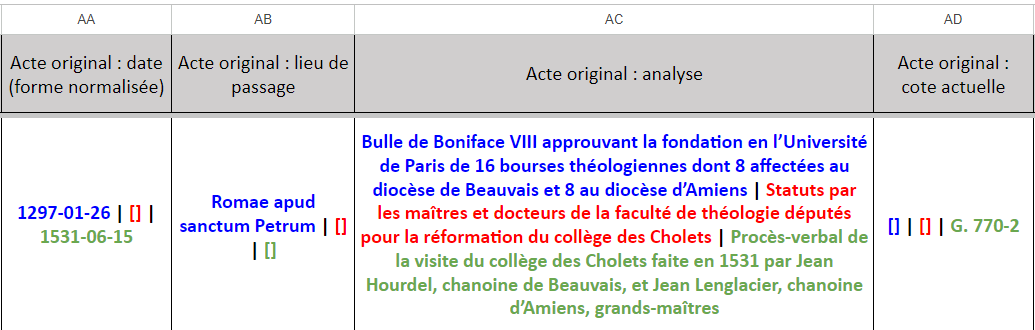
\includegraphics[width=1\linewidth]{images/tableau-positions-originaux.png}
    \caption{Capture d'écran d'une ligne d'un tableau pour illustrer l'importance de la position. Chaque couleur représente un acte.}
    \label{fig:position-tableau-couleur}
\end{figure}
Il en résulte qu'il faut également trouver le moyen de représenter l'absence de valeur. Puisque la position est importante on doit pouvoir la conserver, même quand il y a une valeur nulle ; c'est là qu'intervient une autre chaîne de caractères récurrente formée d'un crochet gauche et d'un crochet droit \textbf{"[]"}  qu'on appellera "crochets vides". Cette chaîne de caractères est utilisée tout au long des dépouillements pour représenter l'absence de valeur, quand une donnée était attendue, afin de respecter le schéma de saisie. 
\par
Un dernier exemple, cette fois-ci concernant les personnes. La méthodologie demande d'extraire les noms des personnes, leurs occupations/activités et leurs rôles par rapport au document analysé (auteur, rédacteur, témoin etc) le tout dans une seule colonne. On a donc l'expression de plusieurs valeurs (puisque qu'il est courant que plusieurs personnes soient impliquées dans un acte) et des valeurs de différentes natures. Pour permettre de retrouver quelle information est de quel type, il a été décidé de les ordonner selon un schéma que doit respecter l'archiviste : celui-ci indique en premier et entre crochets le rôle de la personne, puis son nom et entre parenthèses ses occupations/activités. Comme ces dernières peuvent être multiples et qu'on ne peut pas utiliser une barre verticale, on les sépare par un \# (dièse).
\par
Toutes ces consignes de saisie, indispensables à un tel niveau de granularité, visent à permettre aux traitements automatiques ultérieurs sur les données de produire des résultats de qualité. Mais cela exige une attention accrue de la part de la ou des personnes chargées du dépouillement et de la saisie des données. D'ailleurs requérir un tel niveau d'attention a pu entraîner certaines erreurs, qu'il nous a fallu corriger. Ces erreurs sont inévitables lorsqu'une personne humaine est en charge de la saisie. 